\skriptsection{Fourierreihen}{70ff}
    \skriptsubsection{Orthogonalitätsbeziehungen der Basisfunktionen}{75}
        \begin{tabular}{lll}
            $\int\limits_0^T \cos(n\omega t)\cdot \cos(m\omega t)dt=
            \begin{cases}
            T$ für $n=m=0\\
            \frac{T}{2},$ für $n=m>0\\ 
            0,$ für $n\neq m\\
            \end{cases}$ &
            $\int\limits_0^T \sin(n\omega t)\cdot \sin(m\omega t)dt=
            \begin{cases}
            \frac{T}{2},$ für $n=m\\
            0,$ für $n\neq m\\
            \end{cases}$&
            $\int\limits_0^T \cos(n\omega t)\cdot \sin(m\omega t)dt=0$\\

	$(m,n \in \mathbf{N_0})$ &
	$(m,n \in \mathbf{N})$ &
	$(m \in \mathbf{N_0} ; n \in \mathbf{N})$
        \end{tabular}

	\skriptsubsection{Allgemeine Form}{79}
		Eine periodische Funktion f mit Periode $T>0$, lässt sich durch eine Reihe von
		Sinus- und Kosinusfunktionen darstellen, deren Frequenzen ganzzahlige 
		Vielfache der Grundfrequenz $\omega = 2\pi / T$ sind:
		$$ FR[f(t)] = f(t) =\frac{a_0}{2} + \sum_{n=1}^\infty (a_n \cdot \cos(n \omega t) + b_n
		\cdot \sin(n\omega t))$$
		Die Koeffizienten der Entwicklung von $f(t)$ sind:
		$$ a_n=\frac{2}{T}\int_{0}^{T} f(t) \cdot \cos(n\omega t)\, \mathrm{d}t \quad (n=0,1,2,3,\ldots)
		 \qquad \qquad b_n=\frac{2}{T}\int_{0}^{T} f(t) \cdot \sin(n\omega t)\,
		 \mathrm{d}t \quad (n=1,2,3,\ldots) $$ 
		Der erste Summand der Reihe $a_0/2$ ist der Gleichstromanteil (Mittelwert) von
		$f(t)$ im Intervall $(0,T)$
		$$ a_0=\frac{2}{T}\int_{0}^{T} f(t)\ \mathrm{d}t \quad (n=0)$$

	\skriptsubsection{Komplexwertige Darstellung der Fourierreihen}{95ff}
		$$f(t) = \sum\limits_{k = -\infty}^{\infty} c_k \cdot e^{j k \omega t} \qquad \text{mit} \qquad c_n=\overline{c_{-n}}=\frac{1}{T}\int_0^T{f(t)\cdot e^{-jn\omega t}dt} \qquad (n \in \mathbf{N_0})$$
		\subsubsection{Umrechnungsformeln}
			$$c_n=\overline{c_{-n}}=\frac{a_n-jb_n}{2} (n=0,1,2,3,\ldots\text{ wobei }b_0=0)\qquad
			\left.
			\begin{array}{l} 
				a_n=2Re(c_n) = c_n + c_{-n}\\
				b_n=-2Im(c_n) = j(c_n - c_{-n})
			\end{array}
		    \right\} 
		    \quad \begin{array}{l}
				(n \in \mathbf{N_0}) \\
				(n \in \mathbf{N})
			\end{array}$$ \\
		$c_0 = \frac{a_0}{2} \qquad c_{-n} = \frac{a_n + jb_n}{2}$

	  
	\skriptsubsection{Sätze zur Berechnung der Koeffizienten}{80ff}
		\skriptsubsubsection{Symmetrie}{78}
		Allgemein:$\qquad$ gerade $\cdot$ ungerade $=$ ungerade; $\qquad$ ungerade $\cdot$ ungerade $=$ gerade $\cdot$ gerade $=$ gerade

		\begin{tabular}{l l l l l}
   			Falls $f(t)$ \textbf{gerade} ($ f(-t)=f(t) $) ist &
   			$\Longrightarrow$ & 
			$b_n = 0,$ &
			$a_n = \frac{4}{T} \int\limits_0^{\frac{T}{2}} f(t) \cdot \cos(n \omega t) \mathrm{d}t$ &
			$Im[c_n] = 0$ \\
			
			& & \multicolumn{3}{l} {(achsensymmetrisch: Spiegelung an Y-Achse)}\\
			& & \multicolumn{3}{l} {wenn $f(t)$ gerade ist bezgl. $\frac{T}{4} \Rightarrow a_{2m+1} = 0$}\\
			& & \multicolumn{3}{l} {wenn $f(t)$ ungerade ist bezgl. $\frac{T}{4} \Rightarrow a_{2m} = 0$}\\

			Falls $f(t)$ \textbf{ungerade} ($ f(-t)=-f(t) $) ist &
			$\Longrightarrow$ &
			$a_n = 0,$ &
			$b_n =  \frac{4}{T}\int\limits_0^{\frac{T}{2}} f(t) \cdot \sin(n \omega t) \mathrm{d}t$ &
			$ Re[c_n] = 0$\\

			& & \multicolumn{3}{l} {(punktsymmetrisch: Punktspiegelung im Ursprung)}\\
			& & \multicolumn{3}{l} {wenn $f(t)$ gerade ist bezgl. $\frac{T}{4} \Rightarrow b_{2m} = 0$}\\
			& & \multicolumn{3}{l} {wenn $f(t)$ ungerade ist bezgl. $\frac{T}{4} \Rightarrow b_{2m+1} = 0$}\\
      	\end{tabular}
			 
		\skriptsubsubsection{Linearität}{81}
			$h(t) = r \cdot f(t) + s \cdot g(t) \quad \Longrightarrow \quad a_n^{(h)} = r \cdot
			a_n^{(f)} + s \cdot a_n^{(g)}, \quad b_n^{(h)} = r \cdot b_n^{(f)} + s \cdot b_n^{(g)} \qquad f$, $g$ und $h$ sind T-periodische Funktionen
			
		\skriptsubsubsection{Zeitstreckung/-stauchung ("Ahnlichkeit)}{82}
			$g(t) = f(r \cdot t) $ (mit $ 0 < r \in \mathbb{R}$ ) $\quad \Longrightarrow\quad  
			a_n^{(g)} = a_n^{(f)}, \quad b_n^{(g)} = b_n^{(f)} $ \quad $T^{(g)} = \frac{T^{(f)}}{r} \qquad \omega_g = \frac{2\pi}{T_g}\qquad r\flq1:$Streckung$; r\frq1: $Stauchung
			Zeitspiegelung: $g(t) = f(-1\cdot t) \Longrightarrow \quad a_n^{(g)}=a_n^{(f)}, \quad b_n^{(g)} = sgn(-1)\cdot b_n^{(f)} \qquad $
			
		\skriptsubsubsection{Zeitverschiebung}{84} 
		\label{Fourier_Zeitverschiebung}
		$g(t)=f(t+t_0)$
		$\qquad
		\begin{array}{l}
           a_n^{(g)}=\cos(n\omega t_0)\cdot a_n^{(f)}+\sin(n\omega t_0)\cdot b_n^{(f)}\\
           b_n^{(g)}=-\sin(n\omega t_0)\cdot a_n^{(f)}+\cos(n\omega t_0)\cdot b_n^{(f)}\\
           c_k^{(g)}=e^{jk \omega t_o} \cdot c_k^{(f)}
        \end{array}$
        $\quad
		\begin{array}{l}
           (n=0,1,2,\ldots)  \qquad \text{mit }b_0 = 0 \qquad\\
           (n=1,2,3,\ldots)\\
           (k \in \mathbb{Z})
        \end{array}$
    	$\quad
    	\begin{array}{l}
    		 +t_0$: links$\\
    		  -t_0$: rechts$
    	\end{array}
    	$

\begin{multicols}{2}
	\skriptsubsection{Satz von Dirichlet}{89}
	Die Funktion $f(t)$ sei $T$-periodisch und stückweise stetig mit Limes, dann konvergiert ihre Fourierreihe gegen\\
	$$FR[f(t_0)] = f(t_0) = \frac{f(t_{0-}) + f(t_{0+})}{2}$$
	somit in die Mitte einer Sprungstelle oder den Funktionswert selber.
\vfill\null
\columnbreak
	\skriptsubsection{Abstand f - g}{84}
	Abstand zweier $T$-periodischen, mit Limes stückweise stetigen Funktionen $f$ und $g$.
	$$||f - g|| = \sqrt{\frac{2}{T}\int\limits_0^2[f(t) - g(t)]^2 \mathrm dt} $$
\vfill\null
\end{multicols}

\begin{multicols}{2}
\skriptsubsection{Parsevalsche Gleichung}{97}
$$\frac{a_0^2}{2} + \sum_{n=1}^{\infty}(a_n^2+b_n^2) = \frac{2}{T}\int_{0}^{T}[f(t)]^2dt = ||f||^2$$
$$\sum\limits_{k = -\infty}^{\infty}|c_k|^2 = \frac{1}{T}\int\limits_{0}^{T}[f(t)]^2\mathrm dt$$
\vfill\null
\columnbreak		
\skriptsubsection{Integral und Differential}{88}
Falls die T-periodische Funktion $f$ (auf ganz $\mathbb{R}$) zweimal stetig differenzierbar ist und die Fourierkoeffizienten $a_n$ und $b_n$ besitzt, so gilt:
$$ f'(t) = \sum\limits_{n=1}^{\infty} [b_n n \omega \cdot \cos{(n \omega t)} - a_n n \omega \cdot \sin{(n \omega t)}]$$
$$\int\limits_0^t f(\tau) d\tau = \sum\limits_{n=1}^{\infty} [\frac{b_n}{n \omega}] + 
\frac{a_0}{2} t + \sum\limits_{n=1}^{\infty}
[\frac{a_n}{n \omega} \cdot \sin{(n \omega t)} - \frac{b_n}{n \omega} \cdot \cos{(n \omega t)}] $$
\end{multicols}

\skriptsubsection{Gibbs'sches Phänomen}{92f}
\begin{figure}[htbp]
	\vspace{-\baselineskip}
	\begin{minipage}[c]{8cm}
		Die Fourierreihen schwingen bei Unstetigkeitsstellen über. Die Höhe der grössten überschwingenden Welle
		beträgt 8.94\% der gesamten Sprunghöhe.
	\end{minipage}
	\begin{minipage}[c]{8cm}
		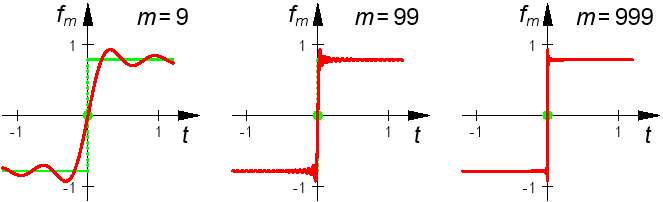
\includegraphics[width=8cm]{./bilder/gibssches_phaenomen.png}  
	\end{minipage}
\end{figure}
\vspace{-\baselineskip}
